\chapter{Foundations of Inference}
\label{SectionFoundationsOfInference}

In section $\ref{sectionNormalDistribution}$, we learnt how to solve problems involving normally distributed populations. In this chapter we will discuss the tools we have for conducting statistical inference on populations that are not normally distributed.

\section{Sampling Distribution}
\label{sectionSamplingDistrib}
\index{Distribution!Sampling distribution}

The concept of sampling distributions is very important for many statistical inference techniques.

\begin{definition}[Point Estimate]
\index{Point estimate}
A point estimate is a single value (i.e. a single point on the real number line) that estimates the value of a parameter.
\end{definition}

In other words, a point estimate is a single value that can be regarded as the best guess of a parameter. A point estimate of $\mu$ is $\bar{x}$ and a point estimate of $\sigma$ is $s$.

\begin{definition}[Sampling Distribution]
\index{Distribution!Sampling distribution}
The distribution of a statistic is referred to as the sampling distribution of the statistic.
\end{definition}

We are particularly interested in the sampling distribution of the sample mean. By this we mean that we are interested in the distribution of $\bar{x}$.


\section{Central Limit Theorem}
\label{sectionCLT}
\index{Central limit theorem}

The \textit{Central Limit Theorem} is an extremely important theorem related to sampling distributions and is of fundamental importance to inferential techniques on the population mean.

\begin{thm}[Central Limit Theorem] \label{theoremCLT}
Consider $m$ random samples, each of fixed size $n$, drawn from a population (following any distribution) with mean $\mu$ and standard deviation $\sigma$. When $m$, the number of samples drawn, is sufficiently large the sampling distribution of the sample mean $\bar{x}$ is approximately normally distributed with mean $\mu_{\bar{x}} = \mu$ and standard deviation $\sigma_{\bar{x}} = \sigma / \sqrt{n}$. That is, $\bar{x} \sim N(\mu,~ \sigma^{2}/n)$.
\end{thm}

\vspace*{-0.5cm}
\begin{figure}[H]
\label{figureCLT}

\noindent
Population Distribution:
\vspace*{-0.25cm}
%\begin{table}[ht]
\renewcommand{\arraystretch}{1.5}% Spread rows out...
%  \begin{tabular}{>{\centering\bfseries}m{1in} >{\centering}m{1in} >{\centering}m{1in} >{\centering \arraybackslash}m{1in}}
\begin{center}
\hspace*{-0.5cm}
\begin{tabular}{	> {\centering}m{1.15in} 
  				> {\centering \arraybackslash}m{1.15in} 
				> {\centering \arraybackslash}m{1.15in} 
				> {\centering \arraybackslash}m{1.15in} 
				> {\centering \arraybackslash}m{1.15in} 
				> {\centering}m{0.2in} }
		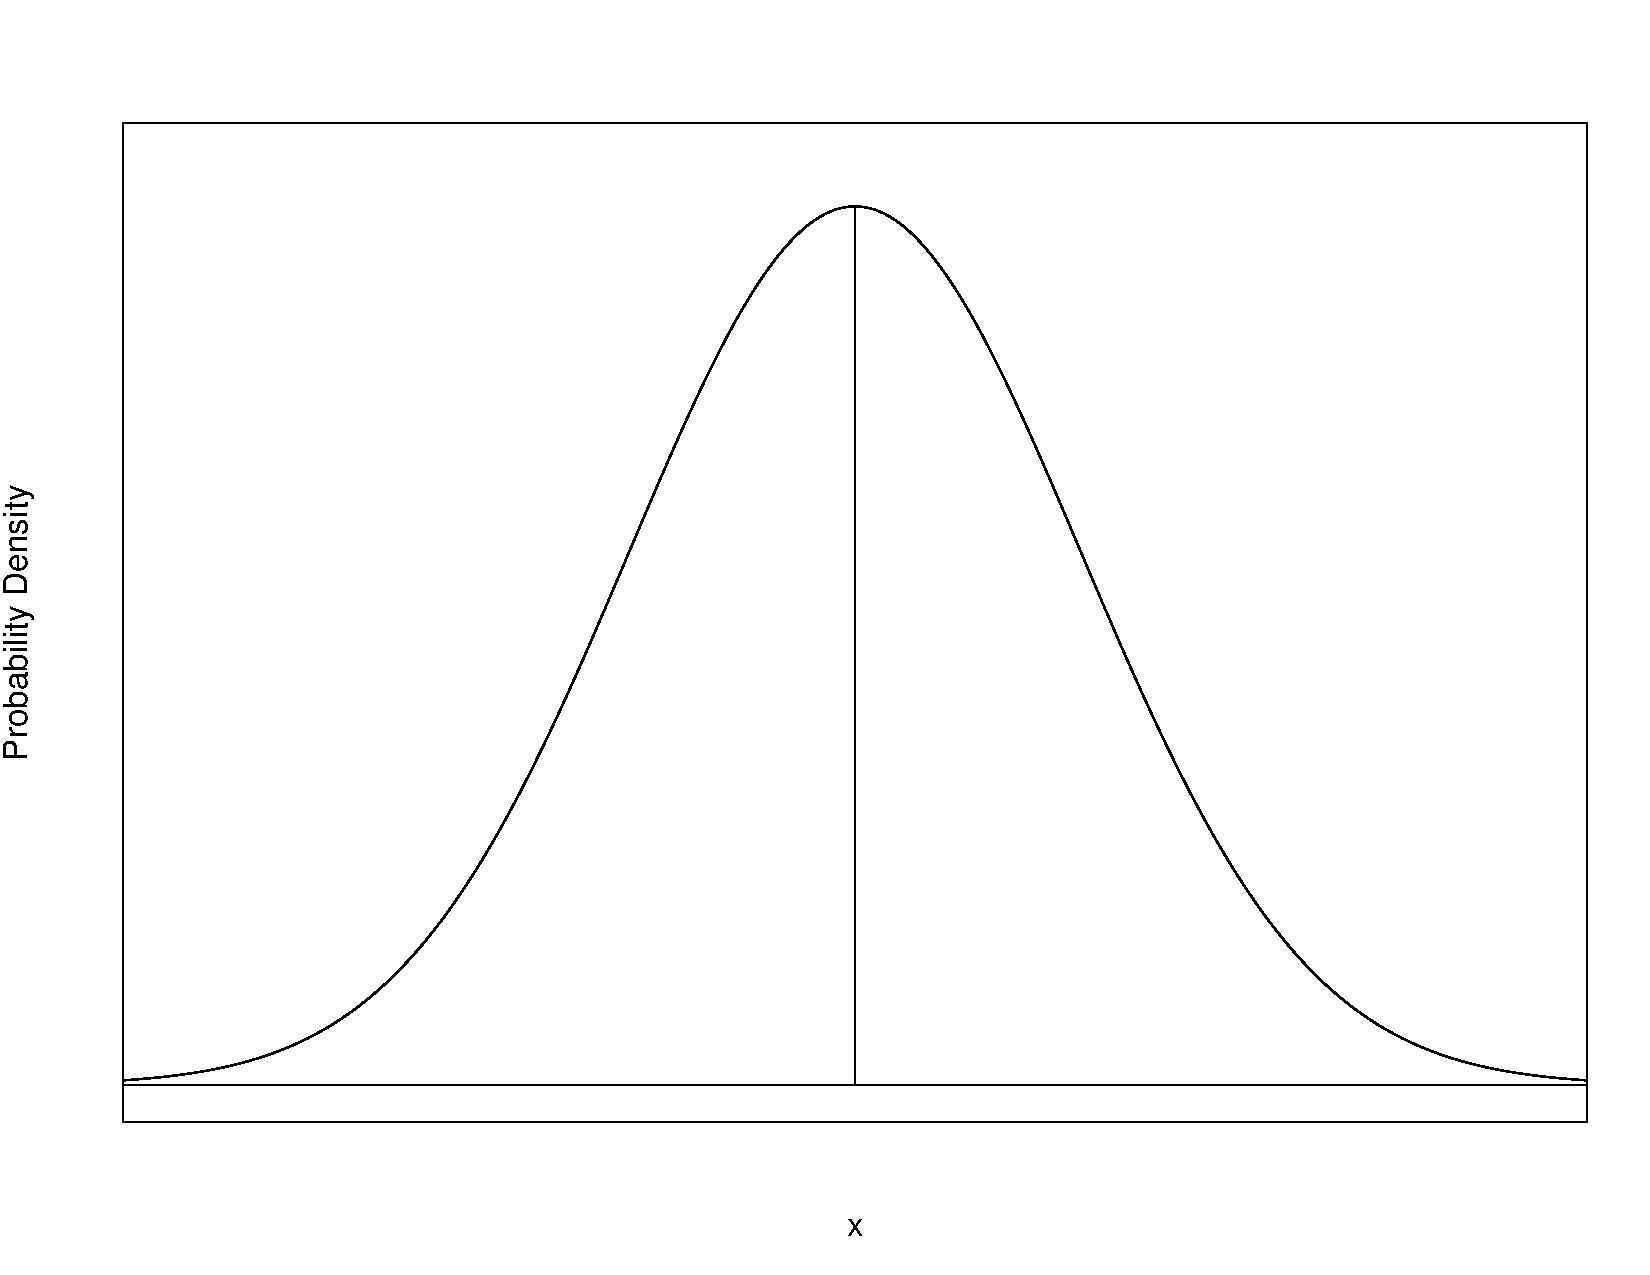
\includegraphics[width=3.00cm]{Section5/density_1.pdf}  
    	&	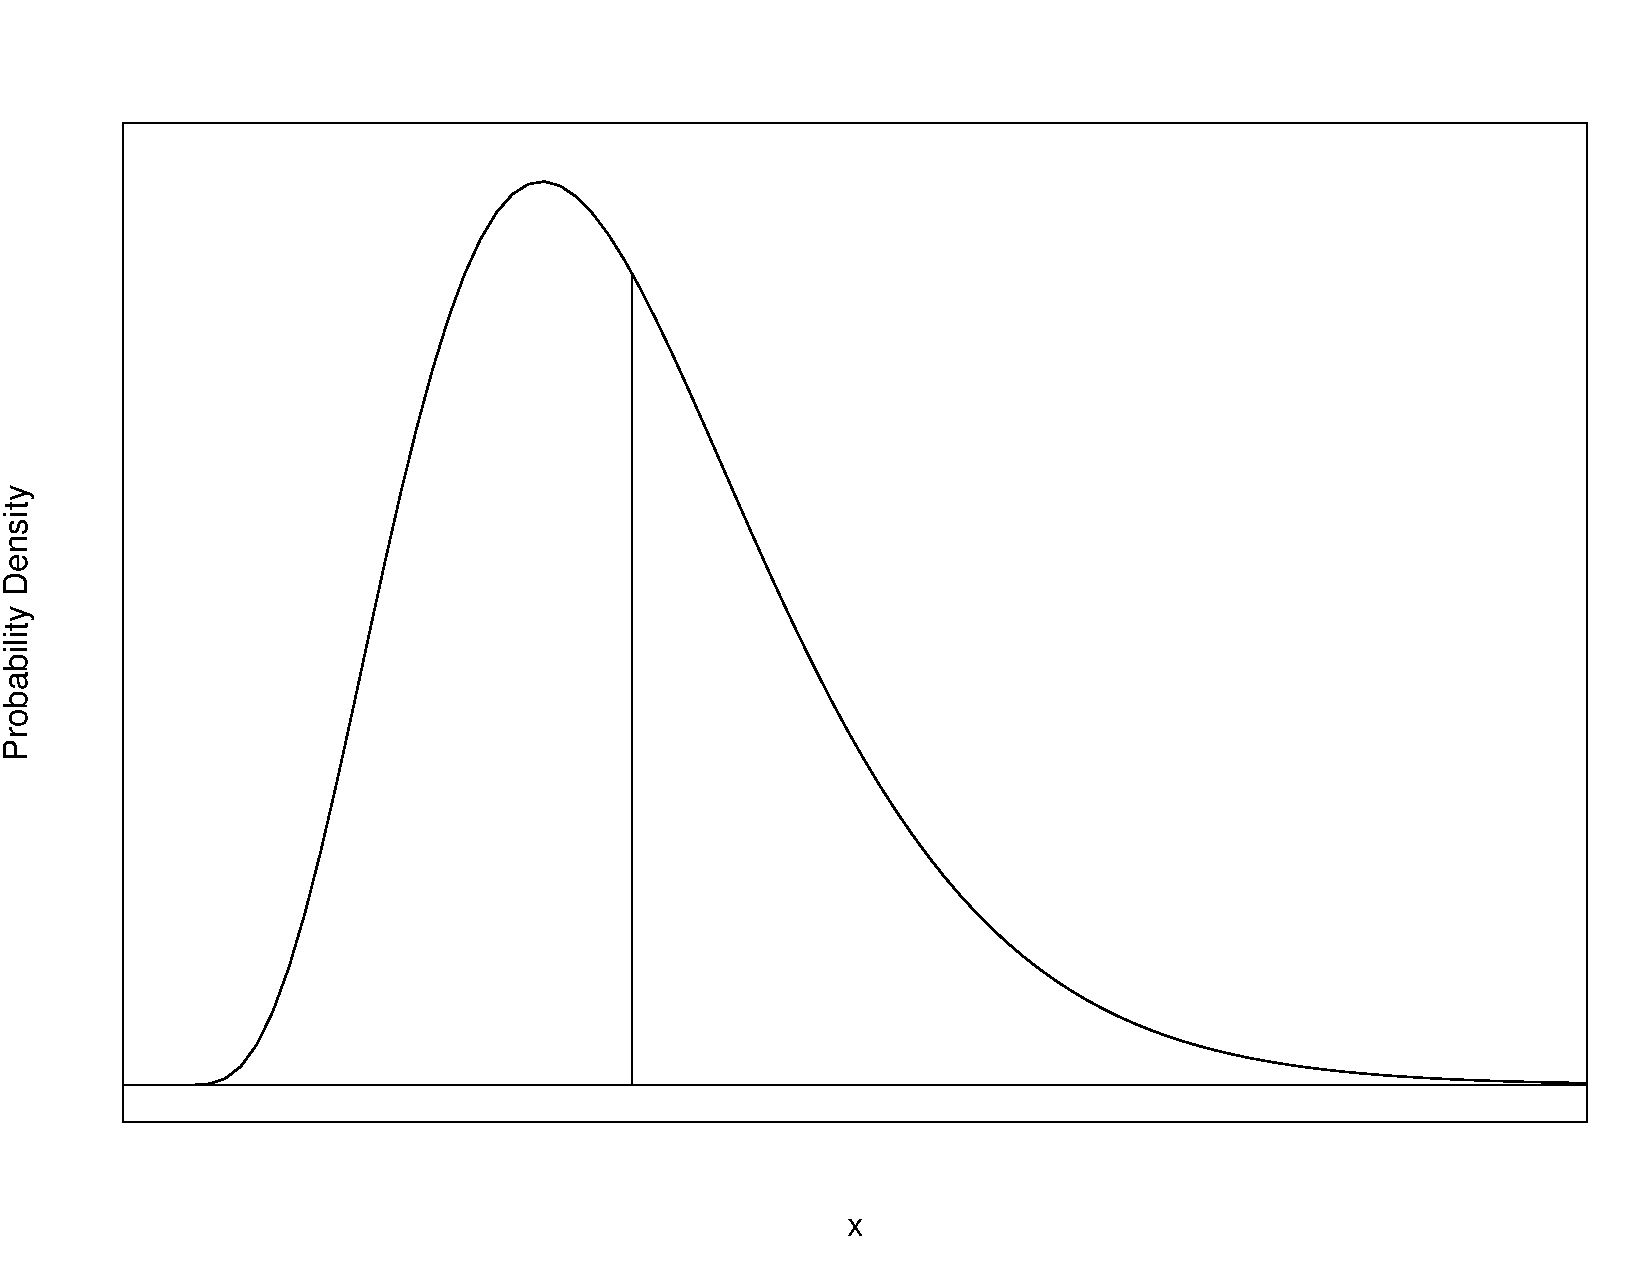
\includegraphics[width=3.00cm]{Section5/density_2.pdf}  
    	& 	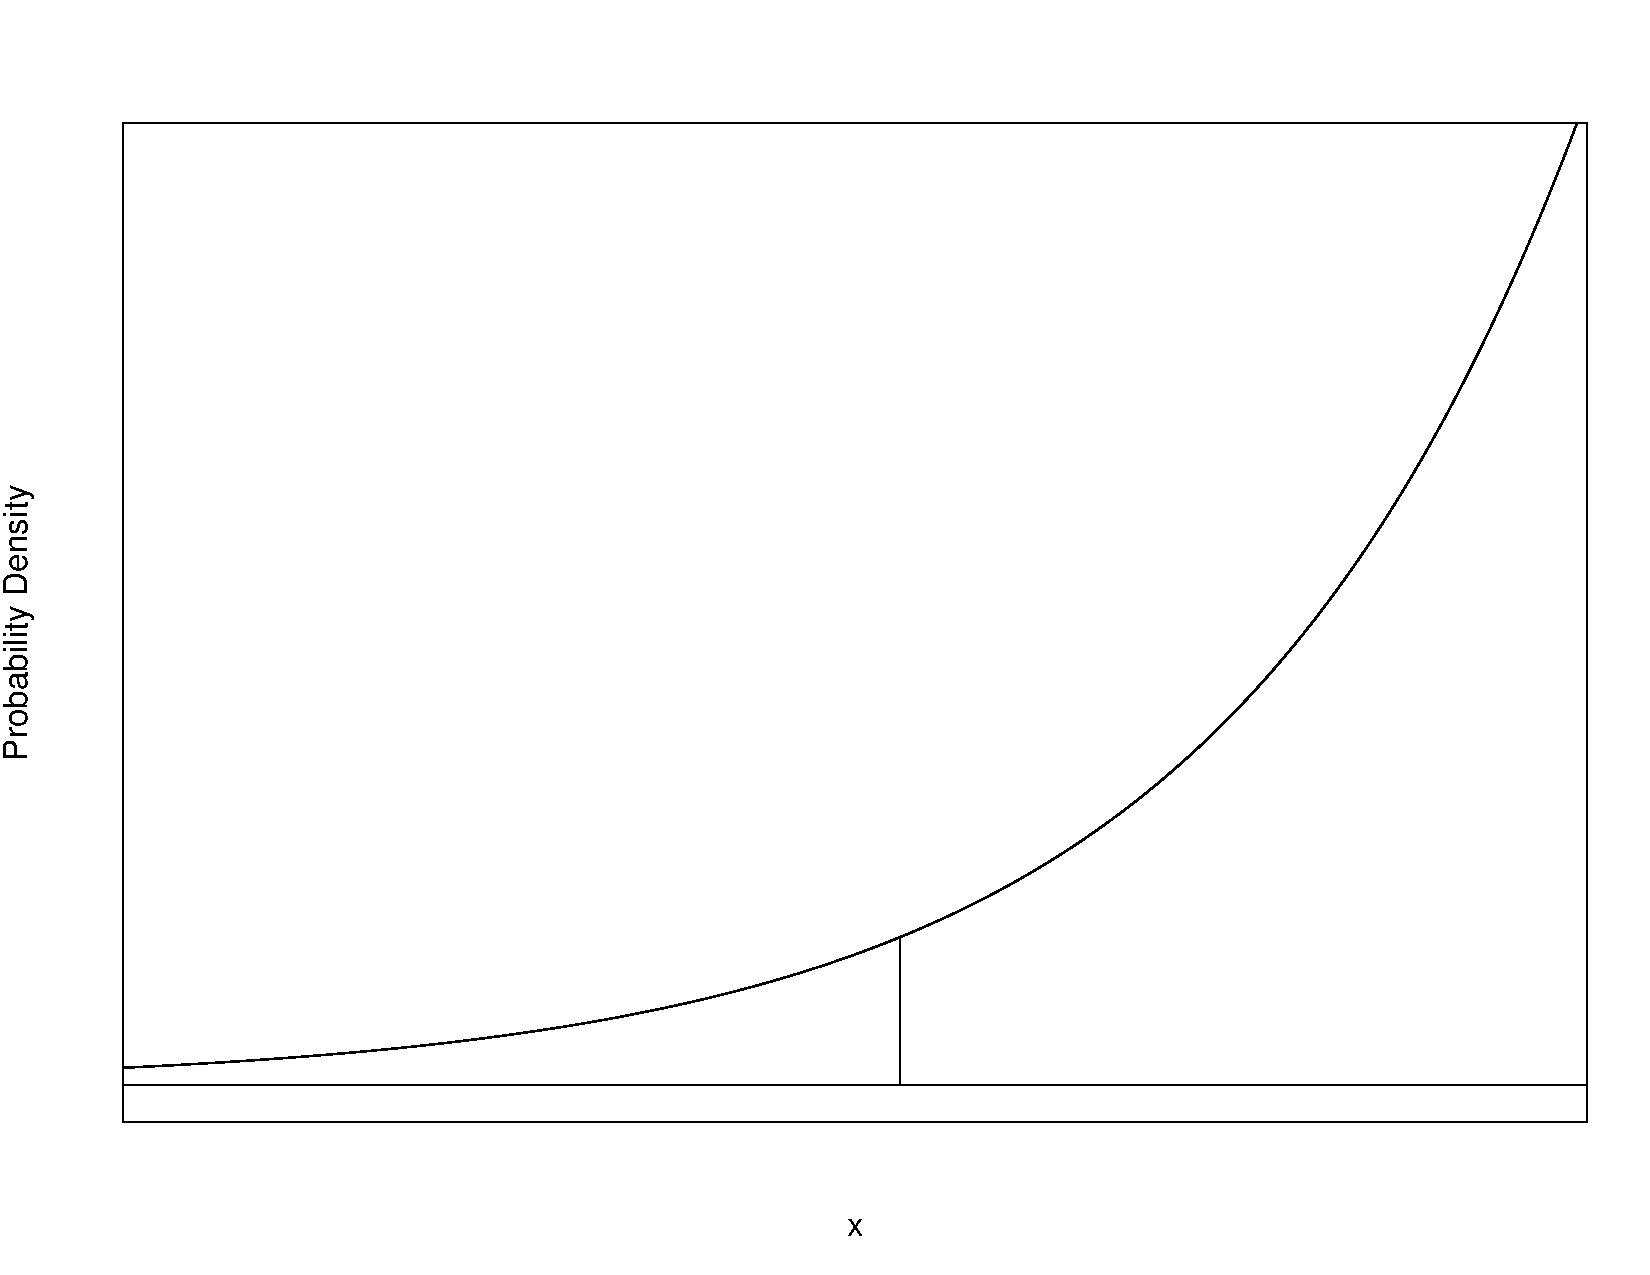
\includegraphics[width=3.00cm]{Section5/density_3.pdf}  
	& 	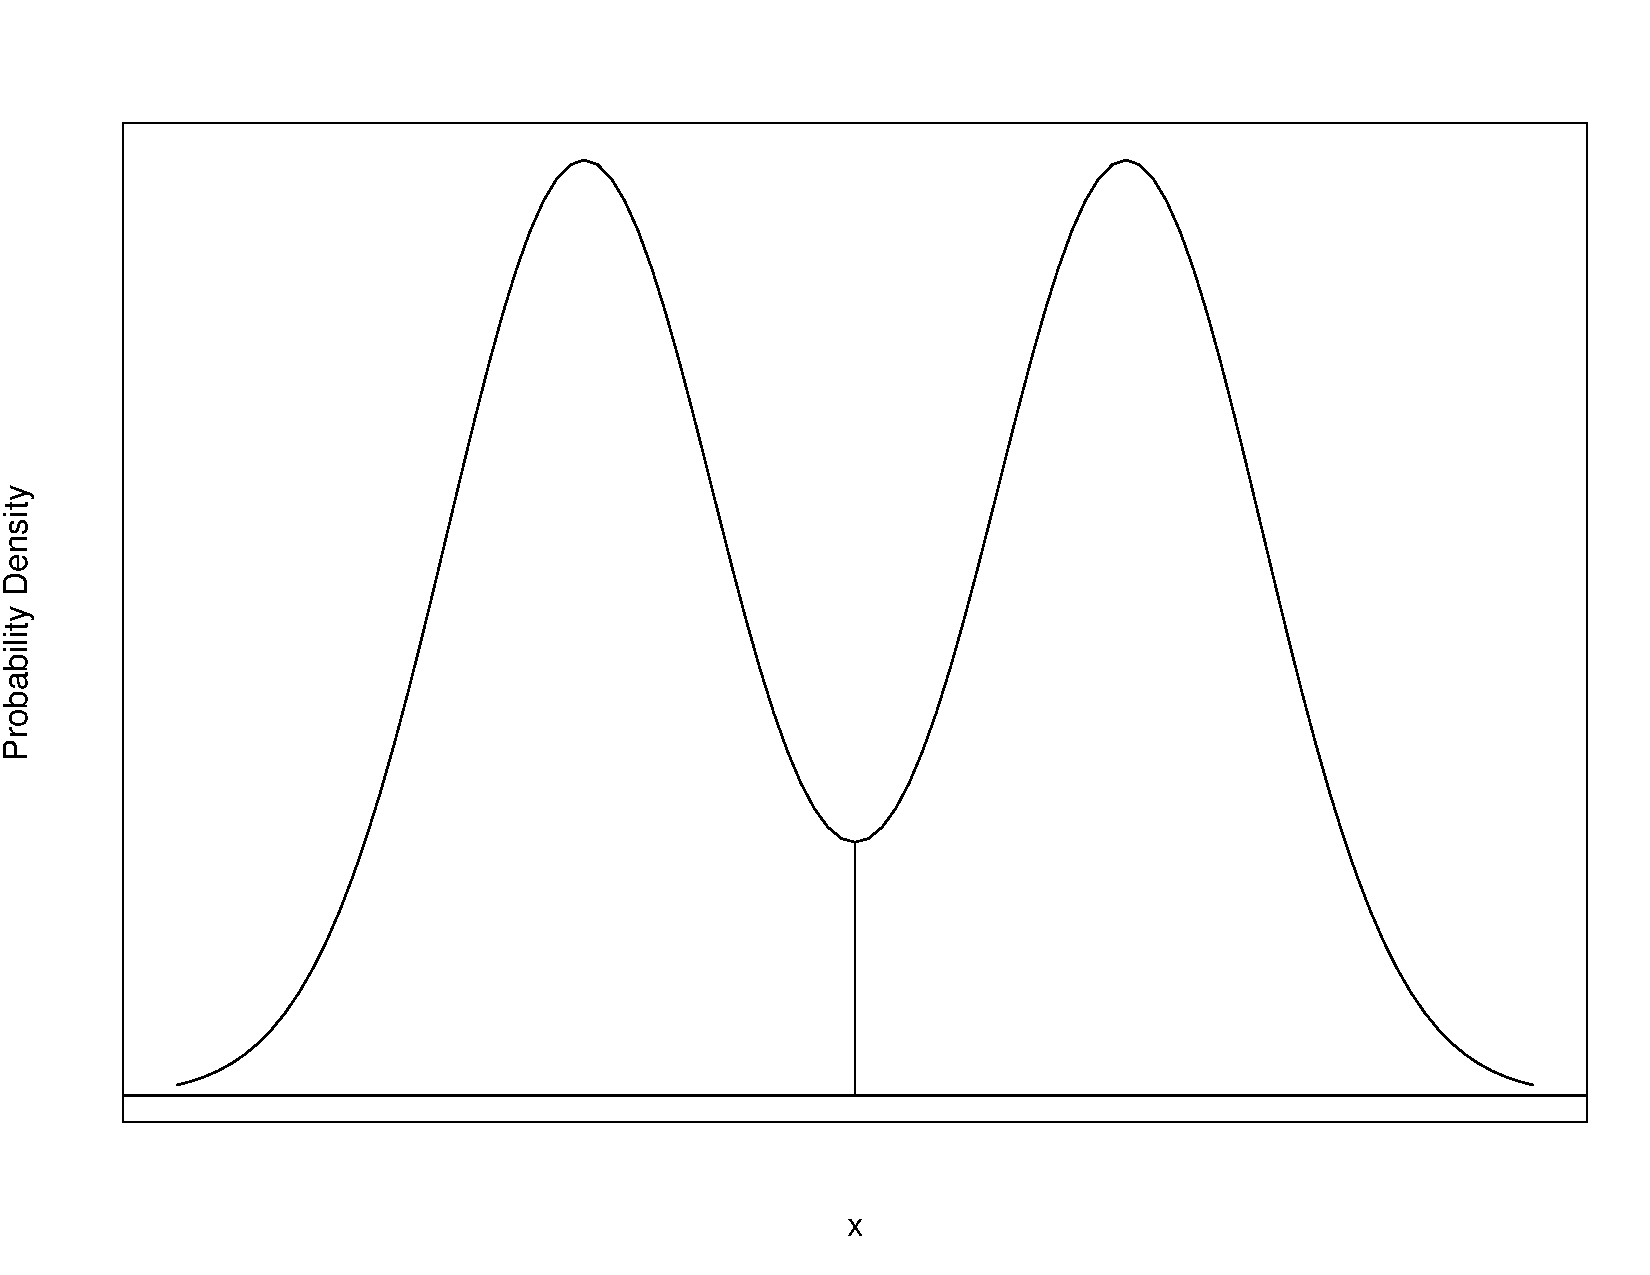
\includegraphics[width=3.00cm]{Section5/density_4.pdf}
	& 	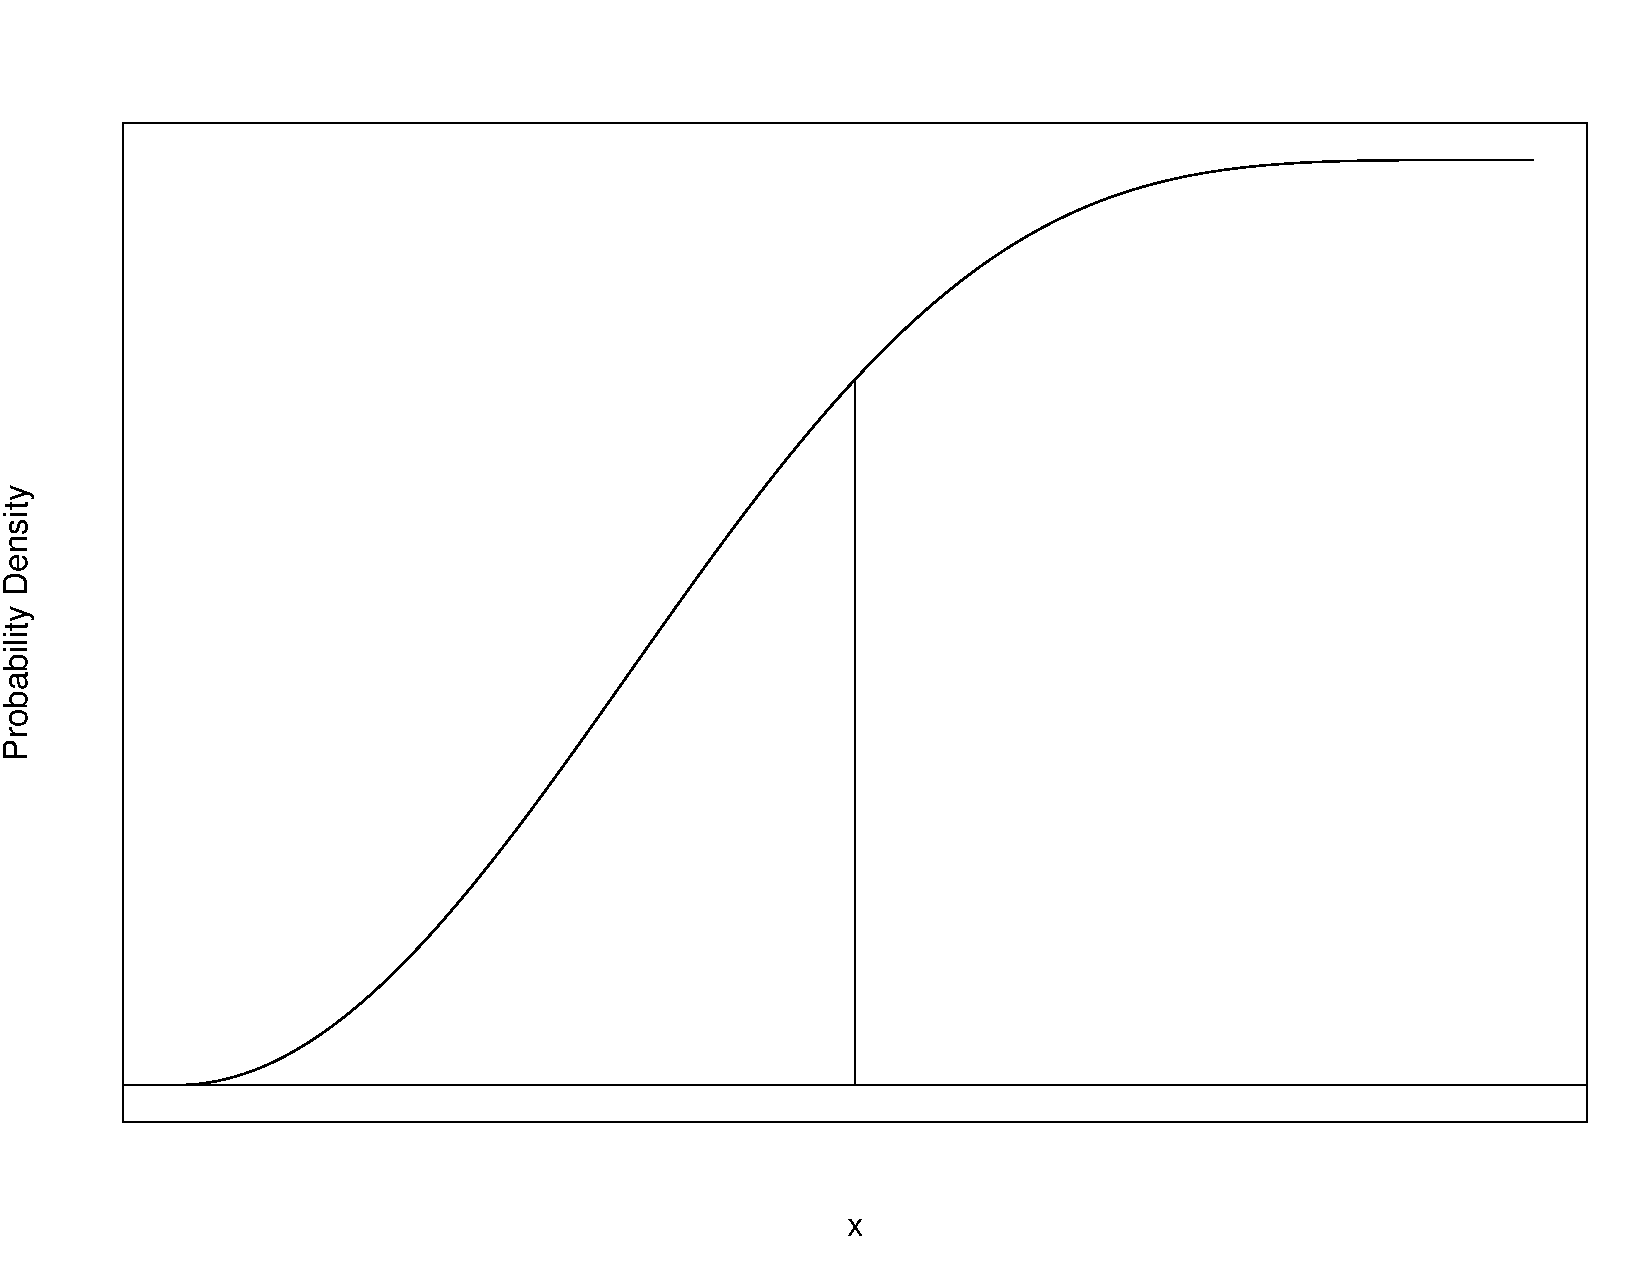
\includegraphics[width=3.00cm]{Section5/density_5.pdf}
    	&	\textbf{$\cdots$} \\
\end{tabular}
\end{center}
%\end{table}



\begin{center}
\begin{tikzpicture}
\hspace{0.50cm} \draw[->] (1,2.5) -- (1, 1.00) ;
%\hspace{0.50cm} \draw[arrow] (1,2.5) -- (1, 1.00) ;
\end{tikzpicture}
\end{center}

\vspace{-0.5cm}
\begin{center}
\begin{tabular}{cccccccccc}
Sample 1	&	Sample 2		& Sample 3	& 	$\cdots$ & $\cdots$ & $\cdots$ \\
-		&	-			&	-		&	$\ldots$ & $\ldots$ & $\ldots$ \\
-		&	-			&	-		&	$\ldots$ & $\ldots$ & $\ldots$ \\
%-		&	-			&	-		&	$\ldots$ & $\ldots$ & $\ldots$ \\
\vdots	&	\vdots		&	\vdots	&	$\cdots$ & $\cdots$ & $\cdots$ \\
%-		&	-			&	-		&	$\ldots$ & $\ldots$ & $\ldots$ \\
-		&	-			&	-		&	$\ldots$ & $\ldots$ & $\ldots$ \\
\hline
\hfill\\[-0.5em]
$\bar{x}_{1}$	&	$\bar{x}_{2}$	&	$\bar{x}_{3}$	&	$\cdots$ & $\cdots$ & $\cdots$ \\
\end{tabular}
\end{center}

\vspace*{-0.1cm}
\hspace{2cm} {\normalsize{Distribution of $\bar{x}$'s:} }
%\vspace{-0.2cm}
%\begin{center}
%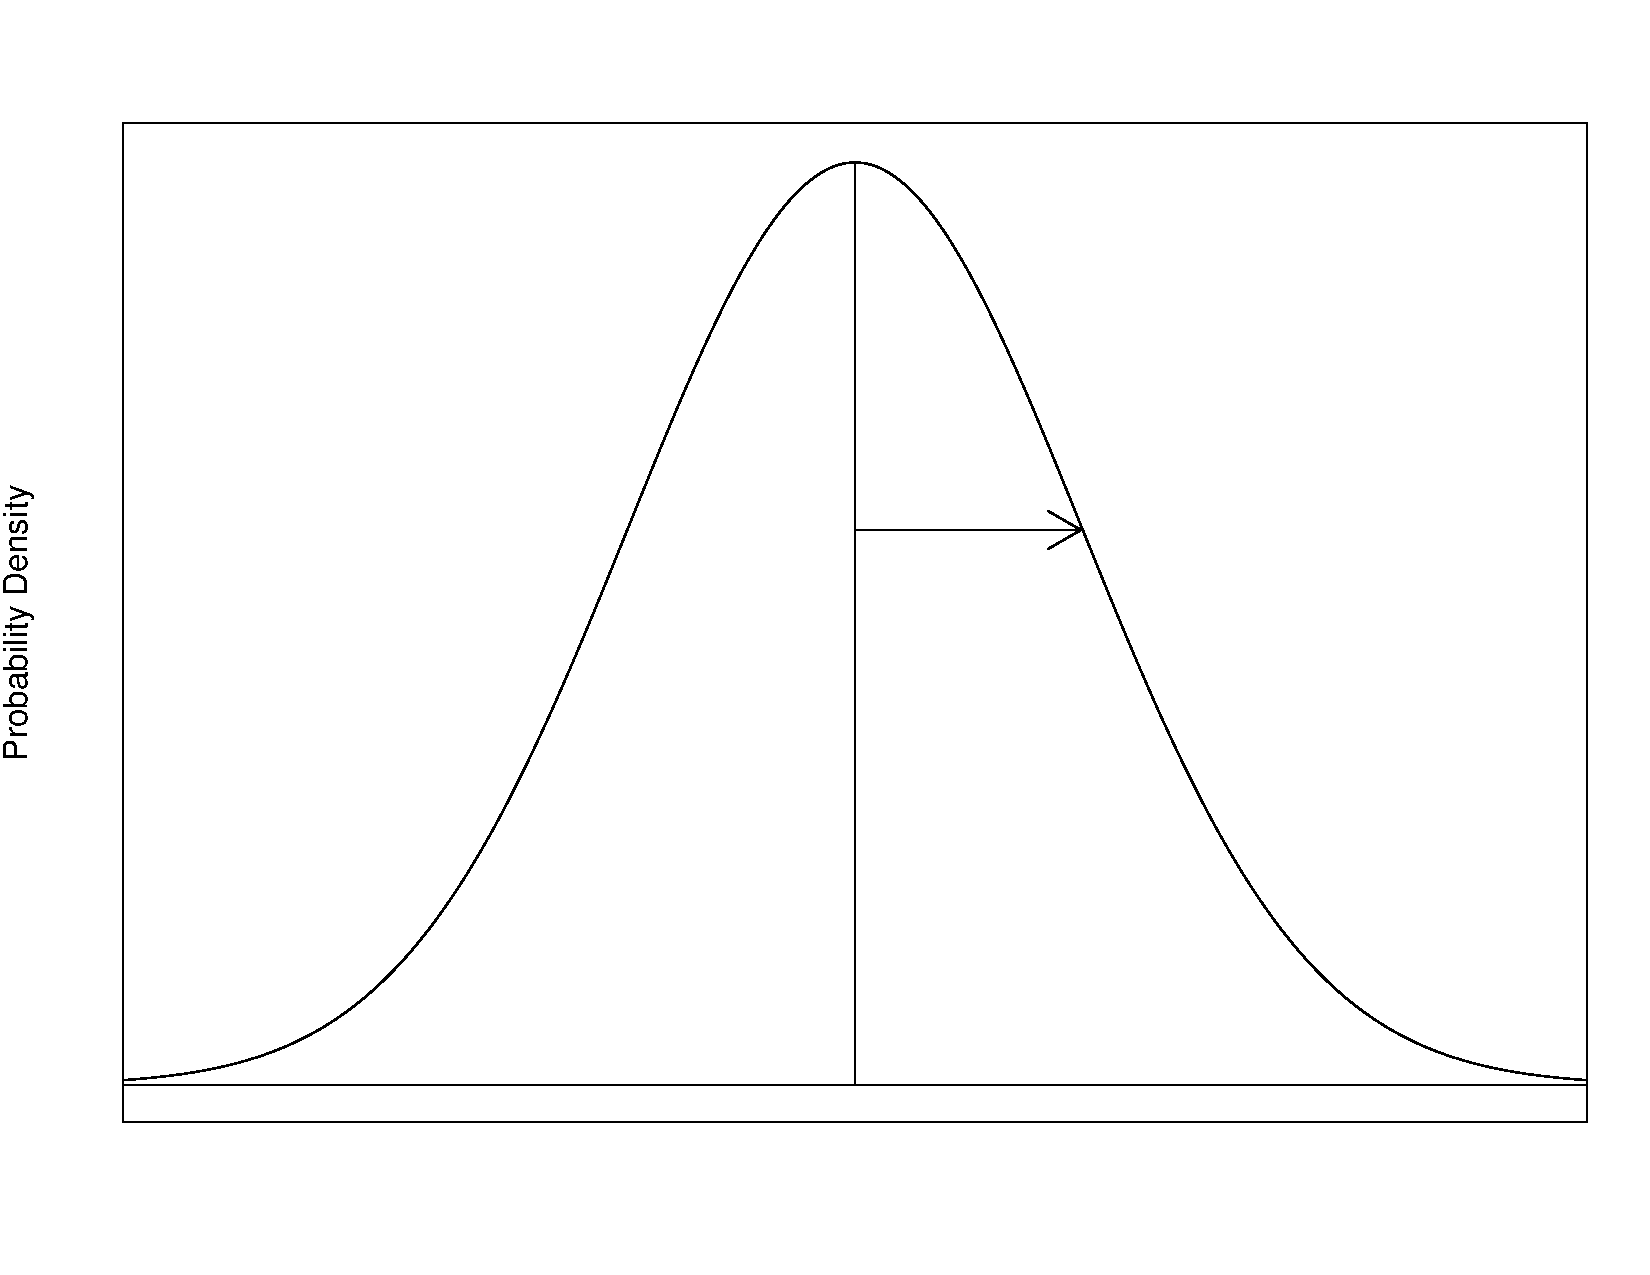
\includegraphics[width=5.00cm]{Section5/dist_x_bar.pdf}
%\end{center}
%
%\vspace*{-0.25cm}
%\begin{center}
%\begin{tabular}{lclccl}
%Mean	& : &	\,~~$\mu_{\bar{x}}$ 		& =	& $\mu$\\
%\hfill\\[-0.75em]
%St. Dev	& : & \,~~$\sigma_{\bar{x}}$	& =	& $\displaystyle\frac{\sigma}{\sqrt{n} }$\\
%\end{tabular}
%\end{center}


%\begin{center}
%\begin{tabular}{cc}
%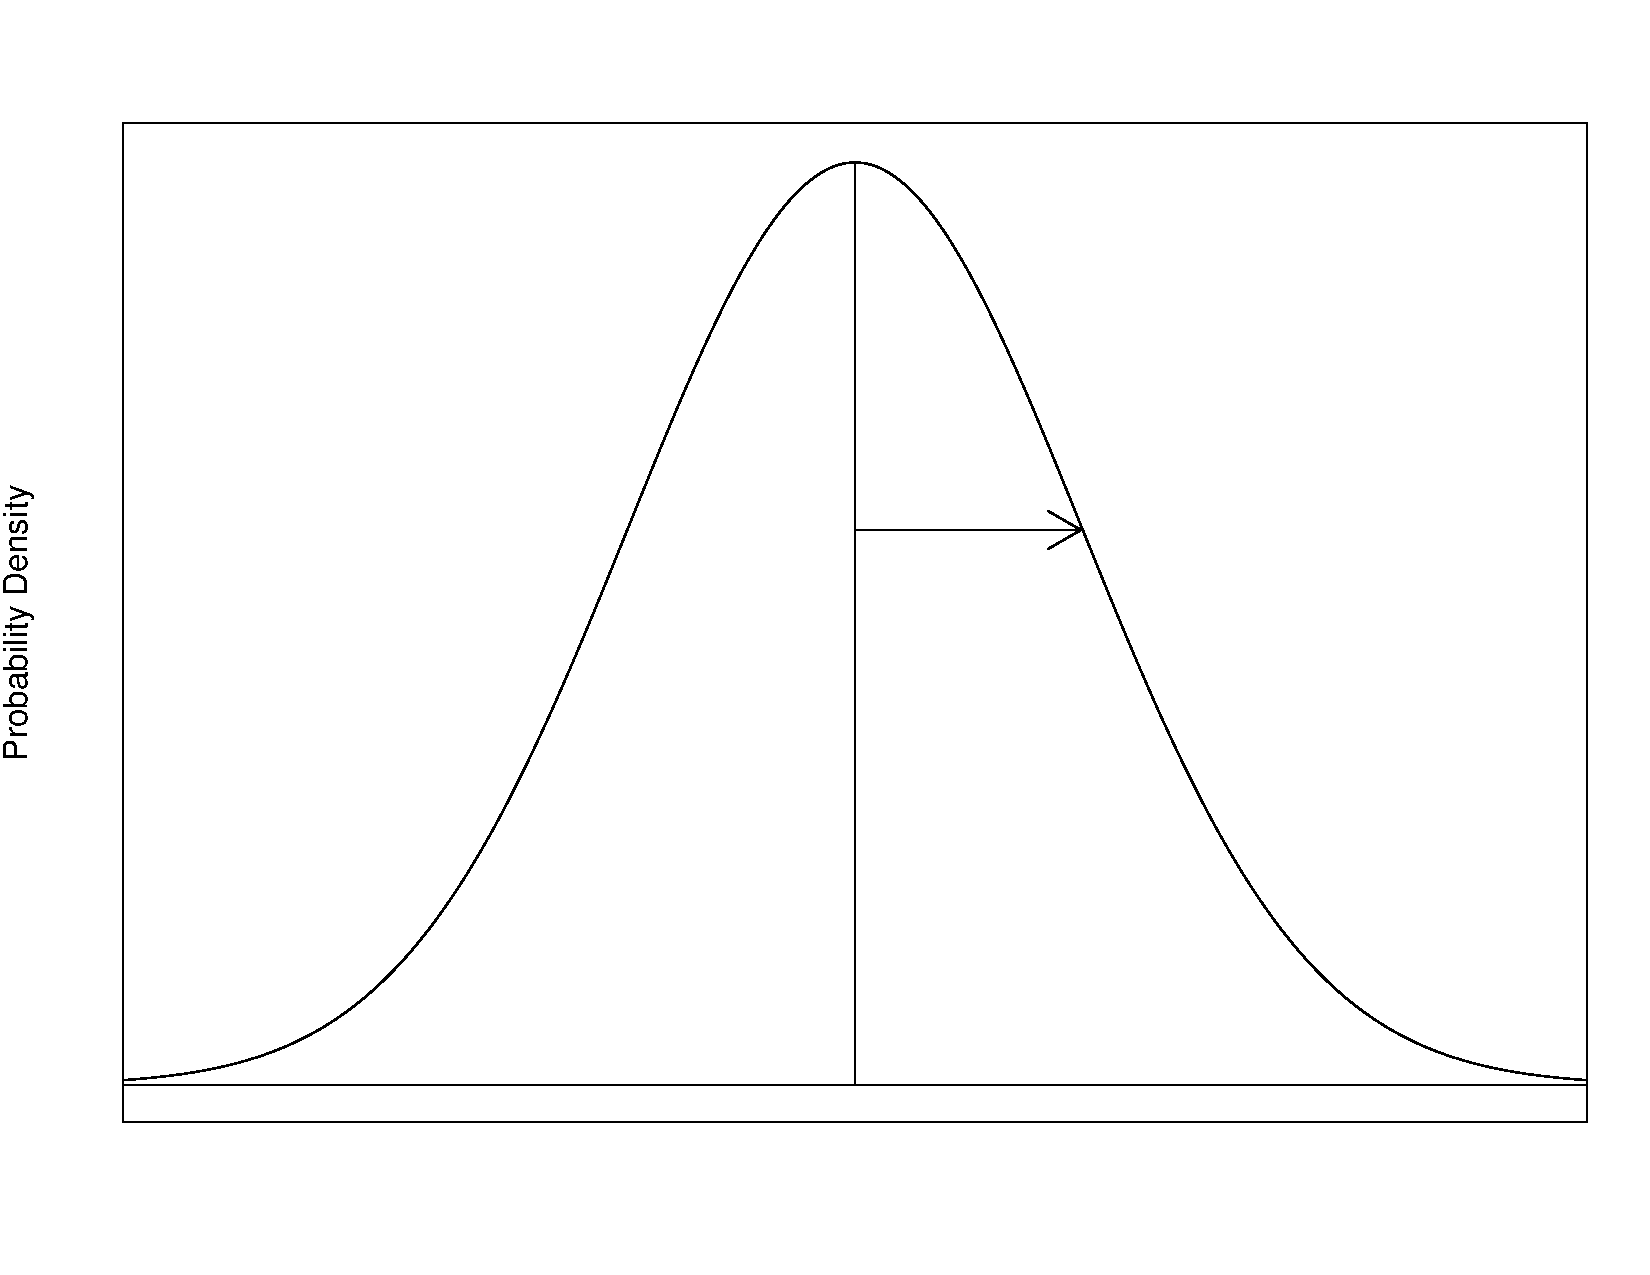
\includegraphics[width=4.50cm]{Section5/dist_x_bar.pdf}	&	\\%Mean :	\\
%\end{tabular}
%%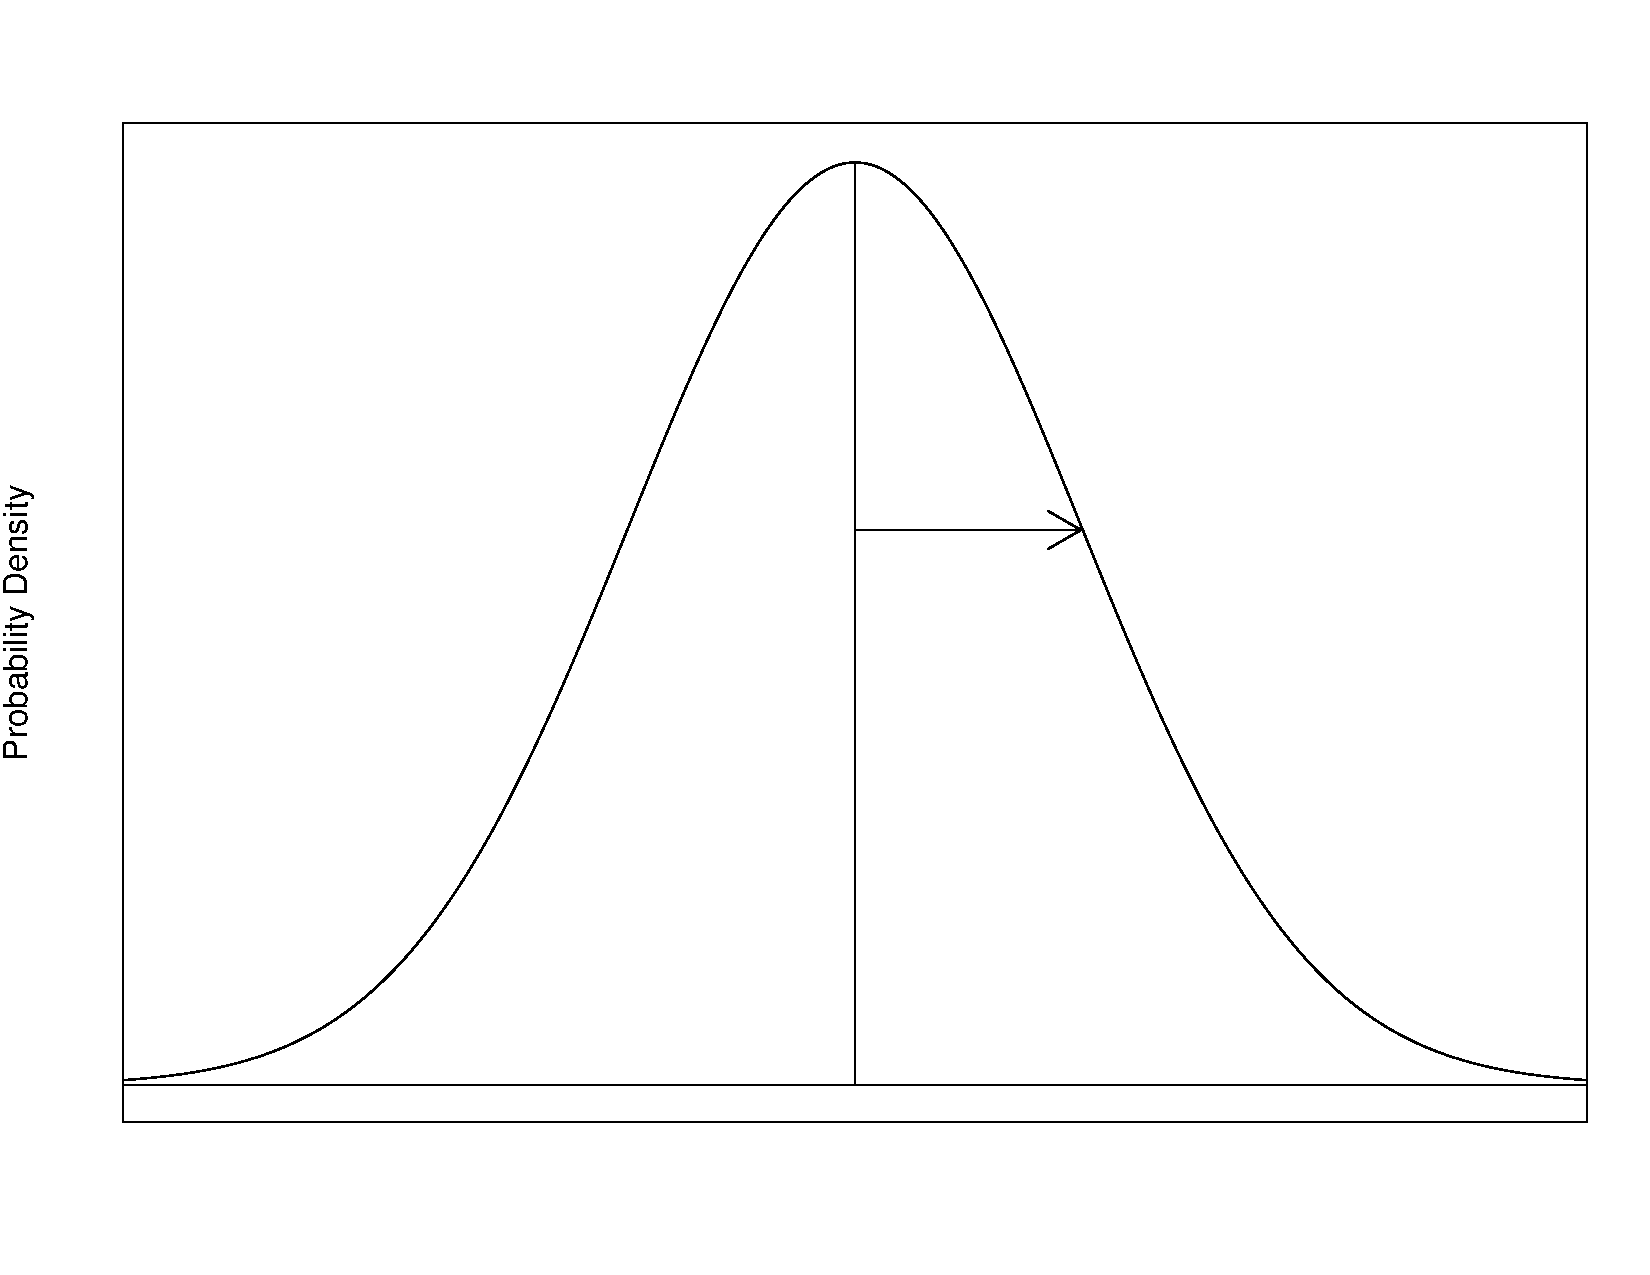
\includegraphics[width=5.00cm]{Section5/dist_x_bar.pdf}
%\end{center}


\begin{center}
\hspace*{5.5cm}
\begin{tabular}{	> {}m{1.5in} 
  				> {\arraybackslash}m{0.2in} 
				> {\flushleft}m{1.5in} }
		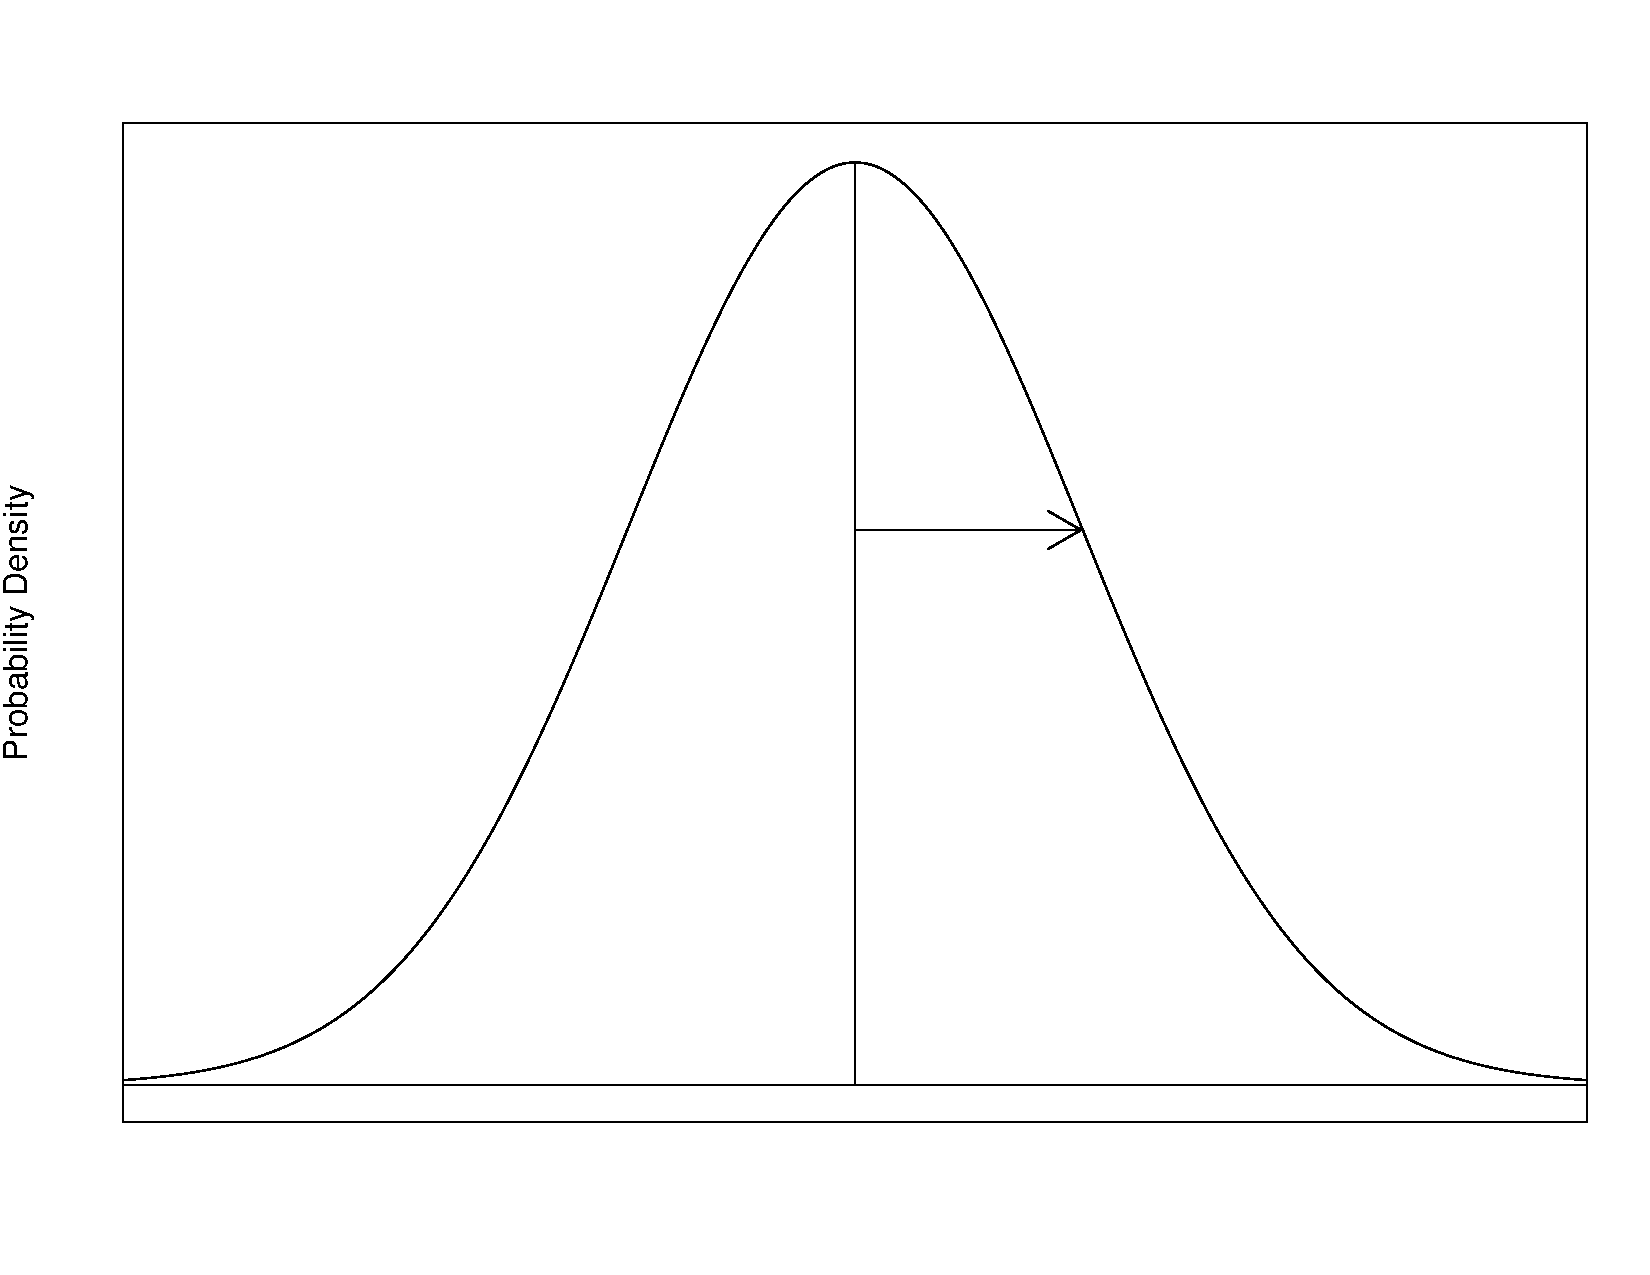
\includegraphics[width=4.00cm]{Section5/dist_x_bar.pdf}  
	&
    	&	Mean : $\mu_{\bar{x}}$  =  $\mu$ \hspace{1in}
		~\hspace*{10in}~
		St. Dev	: $\sigma_{\bar{x}}$	=  $\displaystyle\frac{\sigma}{\sqrt{n} }$\\
\end{tabular}
\end{center}

\vspace*{-0.75cm}
\caption{Implementation of the Central Limit Theorem for creating the 
		sampling distribution of $\bar{x}$.}

\end{figure}



%\begin{tabular}{	> {\centering}m{1.5in} 
%  				> {\arraybackslash}m{0.2in} 
%				> {}m{1.5in} }
%		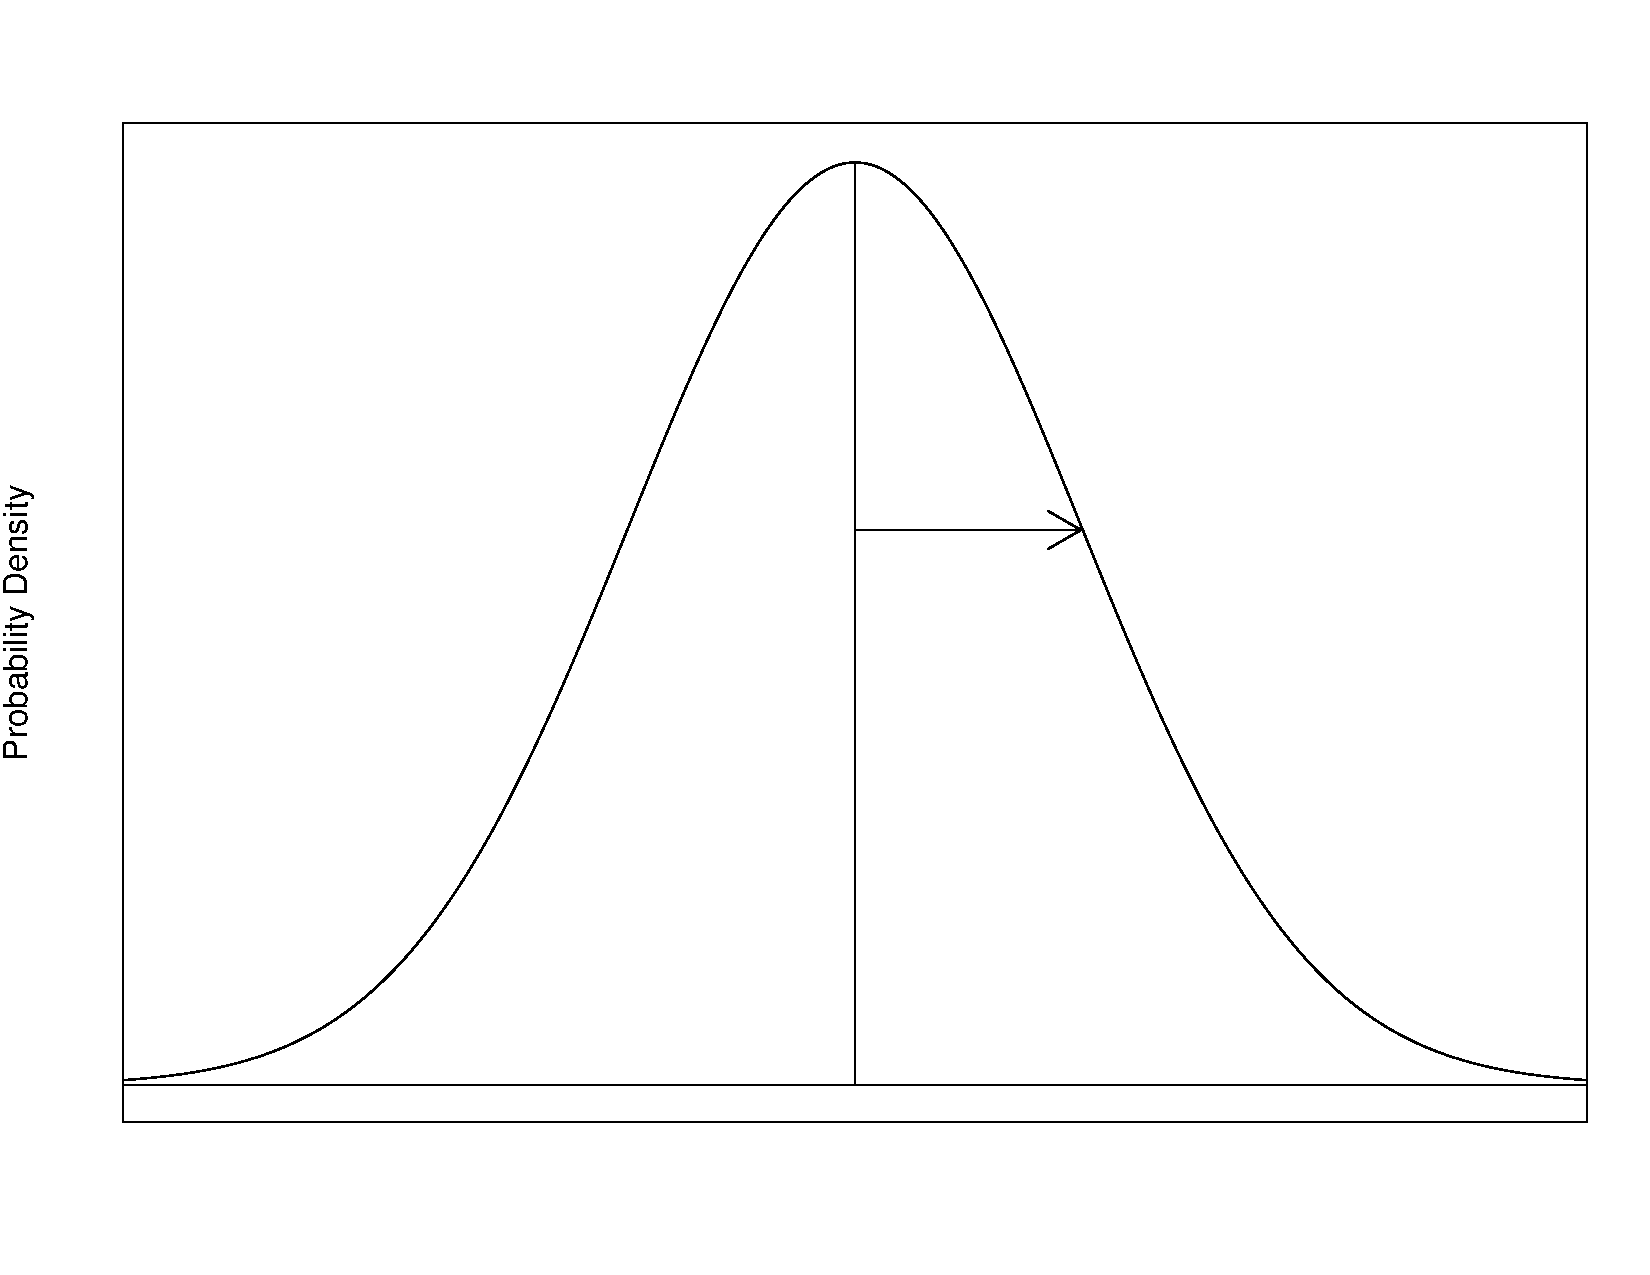
\includegraphics[width=3.00cm]{Section5/dist_x_bar.pdf}  
%	&
%    	&	Mean 	: $\mu_{\bar{x}}$ 	=  $\mu$
%		St. Dev	: $\sigma_{\bar{x}}$	=  $\displaystyle\frac{\sigma}{\sqrt{n} }$\\
%\end{tabular}




$\sigma / \sqrt{n}$ is referred to as the \textit{standard deviation of the sample mean}. This is the standard deviation of $\bar{x}$'s estimate of $\mu$. If we did not know $\sigma$ then we would calculate the standard error of the sample mean using $s$ (the sample standard deviation). We will learn more about these terms in section $\ref{sectionIntroToInference}$. For a better understanding of the manner in which sampling distributions are created it is recommended that the reader should visit an application that can be found at {\em{\ULurl{http://onlinestatbook.com/stat_sim/sampling_dist/index.html}}}. This java applet can be used to visualize various aspects of sampling distributions and how they are affected by the sample size $n$.


\begin{nt}
In order to use the URL above, Java should be installed and enabled in your browser. This application may not work with some browsers (in particular Google Chrome). There are some stability issues and this application may cause your browser to crash, however your computer will not be harmed.
\end{nt}

\begin{example}
Assume $X \sim N(500,90)$. Suppose we take 1000 samples of size $n=25$ from this population. 
Use the central limit theorem to find the distribution of $\bar{x}$.

\hfill\\
{\emph{\textbf{\underline{Solution:}}}}\\


The mean of $\bar{x}$ is
\[ \mu_{\bar{x}}=\mu=500 \]

The standard deviation of $\bar{x}$ is
\[ \sigma_{\bar{x}} = \frac{\sigma}{\sqrt{n}} = \frac{\sqrt{90}}{\sqrt{25}} =6\]

\[\Rightarrow \bar{x} \sim N (500, 36) \]
\end{example}




\section{Introduction to Inference}
\label{sectionIntroToInference}
\index{Inference}

Statistical inference is the study of estimating parameters and quantifying the degree of certainty of each estimate. One of the most important assumptions we make in many inference techniques is the following.

\begin{assumption}[Important Assumption for Inference]
\label{assumptionInferenceParameter}
The value of a parameter is fixed.
\end{assumption}

By assuming the value of a parameter to be fixed, we are assuming that the value of the parameter of interest does not change (at least for the time frame that we are interested in). For instance suppose we are interested in the average salary of all Canadians for the current year. By assumption $\ref{assumptionInferenceParameter}$ it does not matter whether we draw a sample on January 1$^{\text{st}}$ of this year, or on December 31$^{\text{st}}$ of this year or any day in between, the average salary for all Canadians for the current year will not change.\\

Recall that a point estimate is our best single guess for the
estimate of a parameter. However due to the nature of randomness point estimates will likely not be exactly equal to the parameter that they are estimating. Furthermore the value of a point estimate will vary from sample to sample. Thus it is important we are able to quantify the accuracy of point estimates.\\

The standard deviation of the sampling distribution of an estimate (or statistic) indicates how much an estimate deviates from the actual population parameter. In other words, this standard deviation describes the typical error associated with point estimates. As a result, we usually refer to this standard deviation as the
standard error $(SE)$ of an estimate.

\begin{definition}[Standard Error of an Estimate]
\index{Standard error}
The standard error of a point estimate is its associated standard deviation.
\end{definition}

The standard error is used in constructing confidence intervals 
in chapter $\ref{chapterConfidenceIntervals}$
and conducting hypothesis tests in chapter $\ref{chapterHypothesisTests}$.

\begin{nt}
Although estimates usually are not exactly equal to the parameter they are estimating, they become more accurate as more data becomes available (i.e. as the sample size increases). As such we get a smaller standard error as the sample size increases.
\end{nt}
